%
% Acta Acustica united with Acustica -- Instructions for Authors, 2017-03-01
%
\documentclass[twocolumn]{article}

%%%%%%%%%%%%%%%%%%%%%%%%%%%%%%%%%%%%%%%%%%%%%%%
%% Comment / uncomment for one or two column(s) fomat
%\documentclass{article}

\usepackage[modulo,switch]{lineno}
\modulolinenumbers[1]
%%%%%%%%%%%%%%%%%%%%%%%%%%%%%%%%%%%%%%%%%%%%%%%
%% Comment / uncomment for showing line numbers
 \linenumbers

\usepackage[utf8]{inputenc}
\usepackage{amsmath}
\usepackage{amssymb}
\usepackage{float}
\usepackage{graphicx}

\makeatletter\@ifundefined{date}{}{\date{}}
\makeatother

%\markright{\hfill Kergomard {\em et al.}, p.\ }
\pagestyle{myheadings}

\paperheight297mm \paperwidth210mm
\textwidth170mm  \textheight245mm  \oddsidemargin 20mm
\evensidemargin\oddsidemargin \hoffset-22.4mm \voffset-28.4mm
\topmargin0pt \headheight20mm \headsep4mm \topskip0mm
\footskip17.5mm \columnsep7mm \arraycolsep2pt \parindent10pt
\renewcommand{\abstractname}{Introduction}

\begin{document}

\title{TTT4180 Technical Acoustics - Assignment 0}

\author{Nicholas Bresina, Department of Electronic Systems, NTNU Trondheim, Norway \\
nicholdb@stud.ntnu.no}

\maketitle\thispagestyle{empty}

\begin{abstract}
This report describes the equipment and methods used for the recording assignment in the Technical
Acoustics course (TTT4180).
Furthermore it presents the results in form of computed values attained using the recording.
Finally it provides a discussion of the results as well as difficulties encountered in the process.
\end{abstract}

\section{Material and Methods}
\subsection{Recording Site}
The site chosen for this assignment was the intersection by Studentersamfundet, where the main sound sources
are street vehicles or just traffic noise in short.
% TODO insert coordinates as reference

The microphone was setup pointing directly to the intersection, where the closest point of sound generation
was roughly $4\textrm{m}$ away.
Some of the sounds recorded are from sources up to $50\textrm{m}$ and more away from the microphone.

The recording took place on Sunday, 12th September 2021 between 12:45 and 13:45.
The weather was overcast with a slight wind, a temperature of around $11^\circ\textrm{C}$,
and no precipation.
% TODO insert picture

\subsection{Soundscape}
The main component in the traffic noise is the sound the tires emit while driving on the concrete roads.
This is a steady sound for which the intensity increases mostly with higer travelling speeds of the vehicles,
if we neglect the tire type and its condition.

In addition to that there's the rumbling noise of combustion engines.
The major contributors to the perceived loudness of their sound are the size of the cylinders, the RPMs, and
the attenuation from the exhaust pipes.

Afformentioned would likely be categorized as low-frequency noise, especially when the cars are driving slow
with low RPMs.
This is the case for many of the passing vehicles in the recording.
Occasionally there are also mid/high-frequency sounds, like the screeching of brakes or the honking of car horns.

\subsection{Equipment}
The main setup consisted of a handheld recorder with an external microphone connected by cable.

The microphone model used was a Behringer ECM8000 condenser microphone.
Eventhough the wind was not strong, the wind screen was used preventively.

The external microphone was connected to the input of the digital recorder Zoom H5 (Serial No. 212698) with
an XLR cable.
The recorder was set to a sampling rate of $48\textrm{kHz}$ with 24-bit resolution.

The calibrator Brüel \& Kjær Type 4230 (Serial No. 1719650) was used for the generation of the
reference recordings.
It provides 94dB at $1\textrm{kHz}$.
With this calibration source the gain of the recorder was tuned to match roughly $-6\textrm{dB}$.

Although the recorder was transported in the provided hard case for protection, the position of the analog gain
knob had changed from the calibration before and after the recording.
This results in some uncertainity of the calculated SPLs, which is further adressed in Section 
\ref{subsec:recorder}.

\subsection{Calibration}
With the recordings generated by calibrator signal the digital values can be transformed to pressure
values in Pascal.
To achieve this the formulas for sound pressure level (SPL)

\begin{equation}
    p_{rms} = 10^{\left(SPL/20\right)}p_{0}
\end{equation}

and the digital root-mean-square (RMS)

\begin{equation}
    x_{rms} = \sqrt{\frac{1}{N}\sum x^2\left[n\right]}
\end{equation}

are used to generate a scaling factor.
Multiplying this scaling factor to the sampled signal $x[n]$ results in the digital
values now expressing the measured, calibrated pressures values.
This can be written as

\begin{equation}
    p\left[n\right] = \frac{p_{rms,cal}}{x_{rms,cal}}x\left[n\right]\textrm{,}
\end{equation}

where $p_{rms,cal}$ and $x_{rms,cal}$ are the RMS values of the calibrator recording
and $x\left[n\right]$ are the digital values from the 24-bit WAV-file recording.

\subsection{Computation}
After using the reference recording to compute the pressure values, it was possible
to further analyze them by the usual methods including the Fast Fourier Transform
(FFT), 3rd octave bands, and A-weighted 3rd octave bands.

Python was used as the programming language of choice.
The code written provides a small CLI interface to trigger the computations for the
values of interest.

\section{Results}
The following results were produced from a $30\textrm{min}$ piece of the recording, unless stated otherwise.
Due to difference in the gains before and after the recording, the values are given with a $pre$ and $post$ suffix,
indicating calibration with the reference before and after recording respectively.

\begin{description}
\item[SPL total] is calculated using the RMS values of the recording.

\begin{equation}
\begin{aligned}
    L_{p,pre} & = 74.3 \textrm{ dB} \\
    L_{p,post} & = 75.1 \textrm{ dB} \\
\end{aligned}
\end{equation}

\item[SPL for sequences] are calculated for the time constants of $1\textrm{s}$ and $125\textrm{ms}$.

\begin{equation}
\begin{aligned}
    L_{eq,1s,pre} & = 78.0 \textrm{ dB} \\
    L_{eq,1s,post} & = 78.8 \textrm{ dB} \\
\end{aligned}
\end{equation}

\begin{equation}
\begin{aligned}
    L_{eq,125ms,pre} & = 75.5 \textrm{ dB} \\
    L_{eq,125ms,post} & = 76.4 \textrm{ dB} \\
\end{aligned}
\end{equation}

\item[A-weighted SPL total] is computed from the third-octave-band power spectrum adjusted with the weighting
    shown in Fig. \ref{fig:power_spectrum}

\begin{equation}
\begin{aligned}
    L_{p,pre} & = 68.2 \textrm{ dBA} \\
    L_{p,post} & = 69.1 \textrm{ dBA} \\
\end{aligned}
\end{equation}

\item[Power Spectrum] can be seen in Fig. \ref{fig:power_spectrum}.
    It shows a spectrum with constant bandwidth of $1\textrm{Hz}$.
    Summing up all the SPLs from that spectrum then results in

\begin{equation}
\begin{aligned}
    L_{p,pre} & = 74.3 \textrm{ dB} \\
    L_{p,post} & = 75.1 \textrm{ dB} \\
\end{aligned}
\end{equation}

\item[3rd octave bands] spectrum is also displayed in Fig. \ref{fig:power_spectrum}.
    The total SPL calculated from this spectrum is given by

\begin{equation}
\begin{aligned}
    L_{p,pre} & = 74.3 \textrm{ dB} \\
    L_{p,post} & = 75.1 \textrm{ dB} \\
\end{aligned}
\end{equation}

\end{description}

\begin{figure}[H]
    \centering
    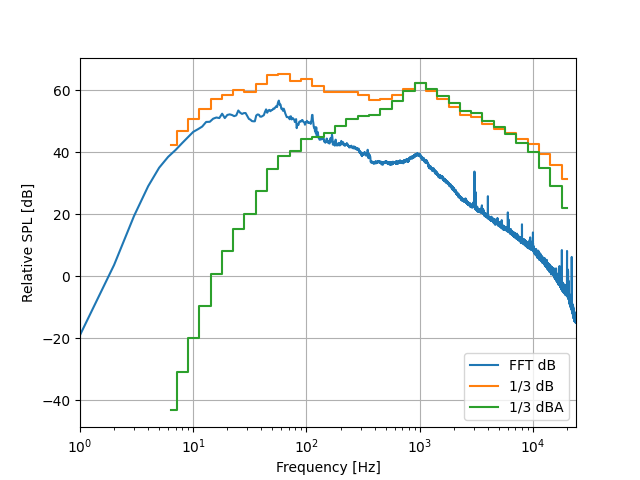
\includegraphics[width=75mm]{./Images/spectrum_plot_step.png}
    \caption{Power Spectrum for the FFT, Third-Octave-Bands, and the A-weighted Third-Octave-Bands using the
    pre-recording reference for calibration}
    \label{fig:power_spectrum}
\end{figure}


\section{Discussion}
\subsection{Recording Site}
% construction site activity + weather
Initially it was planned to record the emitted noise from a construction site.
This turned out to be more difficult than expected.
On the first day of recording, which was a Friday, it was raining heavily.
This resulted in recording mostly rain sounds with some background noise.

In addition to that it's highly reliant on the type of construction that's currently on-going.
There were a number of construction sites as possible candidates.
But on Saturday most of them had a reduced work force and didn't emit a lot of sounds
worth recording.

Which is why we have chosen to switch to the backup plan of recording a traffic intersection.

\subsection{Clipping}
% 1 event of clipping due to incredibly loud motorcycle
With setting the gain of the recorder to correspond to $-6 \textrm{dB}$ using the $94 \textrm{dB}$ source
and the maximum of the recorder being at $+6 \textrm{dB}$ it allows recording SPLs up to $106 \textrm{dB}$.
Even though this is quite loud, there were still a few rare events that caused clipping in the recording,
e.g. a loud motorcycle passing by.


\subsection{Recorder}
\label{subsec:recorder}
% Gain Knobs
One problem already mentioned in earlier sections was the analog gain knob on the recorder.
Although being careful during transport and handling of the recorder, the gain knob was moved.
Because it is unknown at which point during the recording this happened, there's uncertainty
in the validity of the computed values.

The difference between the computed values is approximately $0.8 \textrm{dB}$.
This corresponds to a relativ error of roughly $1\%$, which is significant.


\subsection{Post-Processing}
% length of signal -> RAM
% scaling with 1/N caused by FFT
The most prevalent issue to overcome was the amount of available RAM.
Loading a $30\textrm{min}$ recording and than storing and plotting manipulated copies, like calibrated
signal and power spectrums, quickly filled up the available $8\textrm{Gb}$ of RAM.
Enlarging the virtual RAM and being more thoughtful about ressource usage, helped minimizing this
issue. Allowing to run the code with the complete recording.

\section{Conclusion}
The recording session shows that the noise from traffic intersection ocurring mostly in the lower
frequencies.
At least if accumulated over time the high-frequency content is overshadowed by the low-frequency sounds.

Despite the fact that the power-spectra suggest close to no power in the high frequencies,
those sounds, like the screeching of brakes, are personally perceived a lot more intrusive than the steady
low frequency sounds of the passing vehicles.

Although having the visuals to relate the sounds to is helpful, it should be possible working with an
unattended recording.
Working solely with a time series of sound levels, on the other hand, is more challenging.
This is mainly due to not being able to relate the sound levels to past experiences.
For example if we have a recording, it's possible to listen to the sounds that are
questionable and possibly identify the source.
Which would not be the case using sound levels only.

\section{References}

\end{document}

